Now it is time to tackle non-linear variations of the wave equation in 3+1 dimensions with spherical symmetry. We start by writing the wave equation as
\begin{equation}
    \Box \psi \equiv - \partial_T^2 \psi + \frac{1}{R^2} \partial_R\left( R^2 \partial_R \psi\right) = \mathcal{X} \;,
\end{equation}
where $\mathcal{X}$ is the non-linear term of our equation. Doing a first order reduction followed by the coordinate change to hyperboloidal coordinates, we get
\begin{equation}
    \left\{ \begin{array}{l} 
        \partial_T \Psi = - \Pi \\ 
        \partial_T \Phi = \mathcal{B}\left((r^2 + \Omega^2)^2 \left(H' \partial_r \Phi + \partial_r\Pi\right) + H' L \Omega \left( 2r\Phi - 3 \Omega \Psi + 2 r^{-1} \Omega^2 \Phi\right)\right) + \frac{H'\sqrt{2 L}}{H'^{\,2}-1} \mathcal{X} \\
        \partial_T \Pi = \mathcal{B}\left((r^2 + \Omega^2)^2 \left(\partial_r \Phi + H' \partial_r\Pi\right) + L \Omega \left( 2r\Phi - 3 \Omega \Psi + 2 r^{-1} \Omega^2 \Phi\right)\right) + \frac{\sqrt{2 L}}{H'^{\,2}-1} \mathcal{X}
        \end{array} \right. \; ,
\end{equation}
%
where we used the previous definition for $\mathcal{B}$. We can now substitute $\mathcal{X} = (\Psi /\chi)^3$ to obtain the cubic wave equation. 

Differently from the linear case, where we expect gaussian initial conditions that only differ by amplitude to behave similarly, in the non linear case, we expect that parameter to highly influence the solution. We will investigate this by solving the cubic wave equation with different initial conditions and comparing the results. Solving the cubic wave equation using the same boundary conditions as in the linear case, and using the initial conditions

\begin{equation}
    \begin{array}{c c c c}
        \psi(0,r) = A \, e^{-C \, r^2/2} \; , & \Phi(0,r) = - A \,C \, r \, \frac{\Omega^2(r)}{L(r)} \, e^{-C \, r^2/2} & \text{and} & \Pi(0,r) = 0
    \end{array} \; ,
    \label{eq:cubic_wave_equation-2nd_order_initial_conditions}
\end{equation}
%
with $A = 1.0$ for one of the runs and $A = 10.0$ for the other, while keeping $C = 10$ we get the results shown in figure \ref{fig:cubic_wave_eq}. We can see that, for $A = 1$, we get a solution that behaves very similarly to the linear case, as the wave starts to disperse. Differently from the linear case however, it takes longer to disperse as there is a source term. For $A = 10$, we get a solution that grows rapidly until it explodes.

\begin{figure}[h]
    \centering
    \begin{subfigure}[b]{0.45\textwidth}
        \centering
        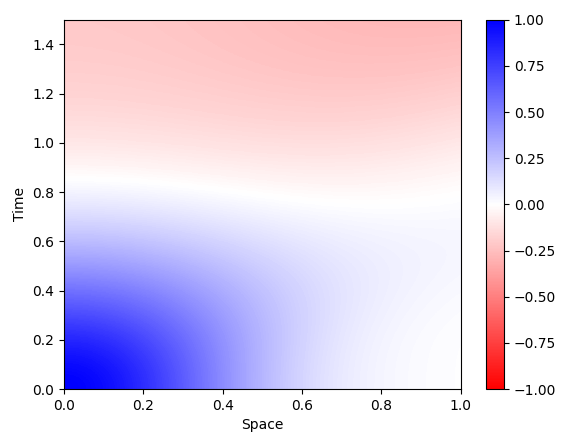
\includegraphics[width=\textwidth]{Images/Cubic_Wave_Equation_3+1_Spherical-A=1-Solution.png}
    \end{subfigure}
    \hfill
    \begin{subfigure}[b]{0.45\textwidth}
        \centering
        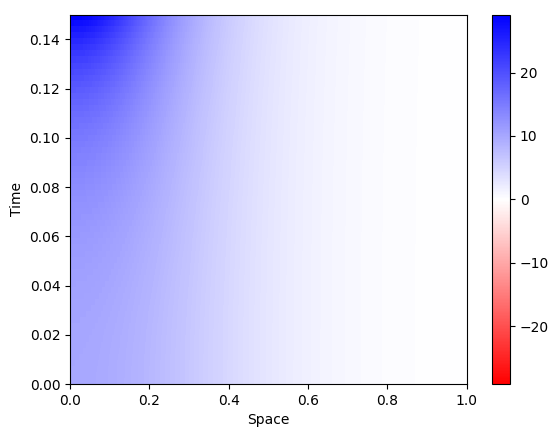
\includegraphics[width=\textwidth]{Images/Cubic_Wave_Equation_3+1_Spherical-A=10-Solution.png}
    \end{subfigure}
    \caption{Evolution of the cubic wave equation in 3+1 dimensions with spherical symmetry using hyperboloidal coordinates with the initial conditions given in equation \eqref{eq:cubic_wave_equation-2nd_order_initial_conditions}. On the left, we have $A=1$ and $C=10$. On the right, we have  $A=10$ and $C=10$.}
    \label{fig:cubic_wave_eq}
\end{figure}

Despite this rapid grouth, our solution still converges cleanly both in the norm and pointwise convergence up until the analytical blowup. This is shown in figure \ref{fig:cubic_wave_eq_convergence} for the case where $A = 10$. 

\begin{figure}[h]
    \centering
    \begin{subfigure}[b]{0.45\textwidth}
        \centering
        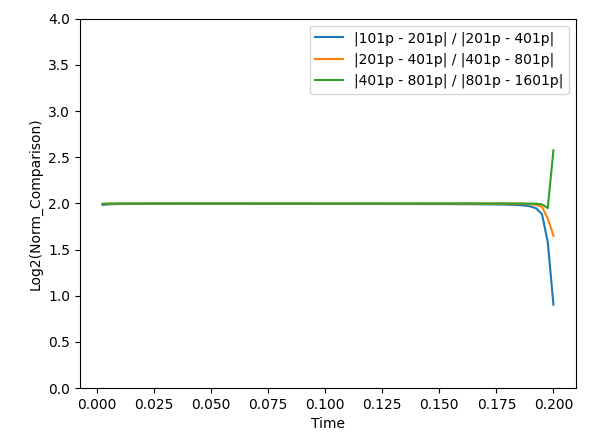
\includegraphics[width=\textwidth]{Images/Cubic_Wave_Equation_3+1_Spherical-A=10-Norm.png}
    \end{subfigure}
    \hfill
    \begin{subfigure}[b]{0.45\textwidth}
        \centering
        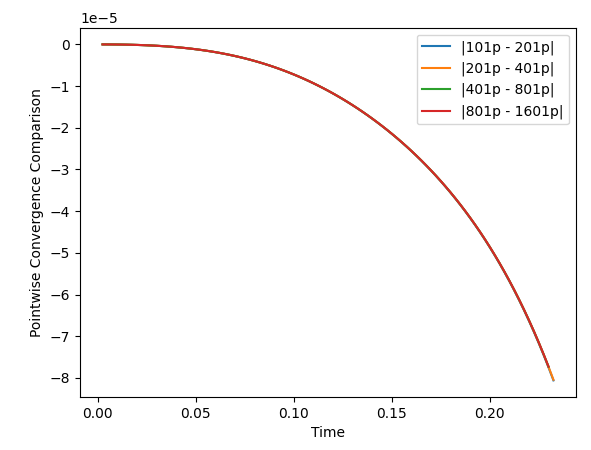
\includegraphics[width=\textwidth]{Images/Cubic_Wave_Equation_3+1_Spherical-A=10-Pointwise.png}
    \end{subfigure}
    \caption{Convergence tests of the evolution of the cubic wave equation in 3+1 dimensions with spherical symmetry using hyperboloidal coordinates, provided the initial conditions given in equation \eqref{eq:cubic_wave_equation-2nd_order_initial_conditions}, with $A=10$ and $C=10$. On the left, we have the $L^2$ norm convergence, and on the right, we have the pointwise convergence at $\mathscr{I}$.}
    \label{fig:cubic_wave_eq_convergence}
\end{figure}